% \levelC{Models}
For each file type, a new model is trained to classify a fragment into two classes, random or structured. The stopping condition used is 10 epochs without improvement at validation accuracy.
The same sampling, input, and output details described in section \ref{sec:evalmodels} were used here. The model identified as ``CM'' was selected to be used.


% \levelC{Dataset}
The model training was divided into two passes, depicted in figure \ref{fig:randommeasure}. Each pass trains a different model for each filetype. In the first pass, the dataset creation for a given file type follows almost the same procedure mentioned in the previous section, but instead of selecting two file types, it selects one file type and uses a random data generator for the other class.

\noindent
\begin{figure*}[htb!]
\centering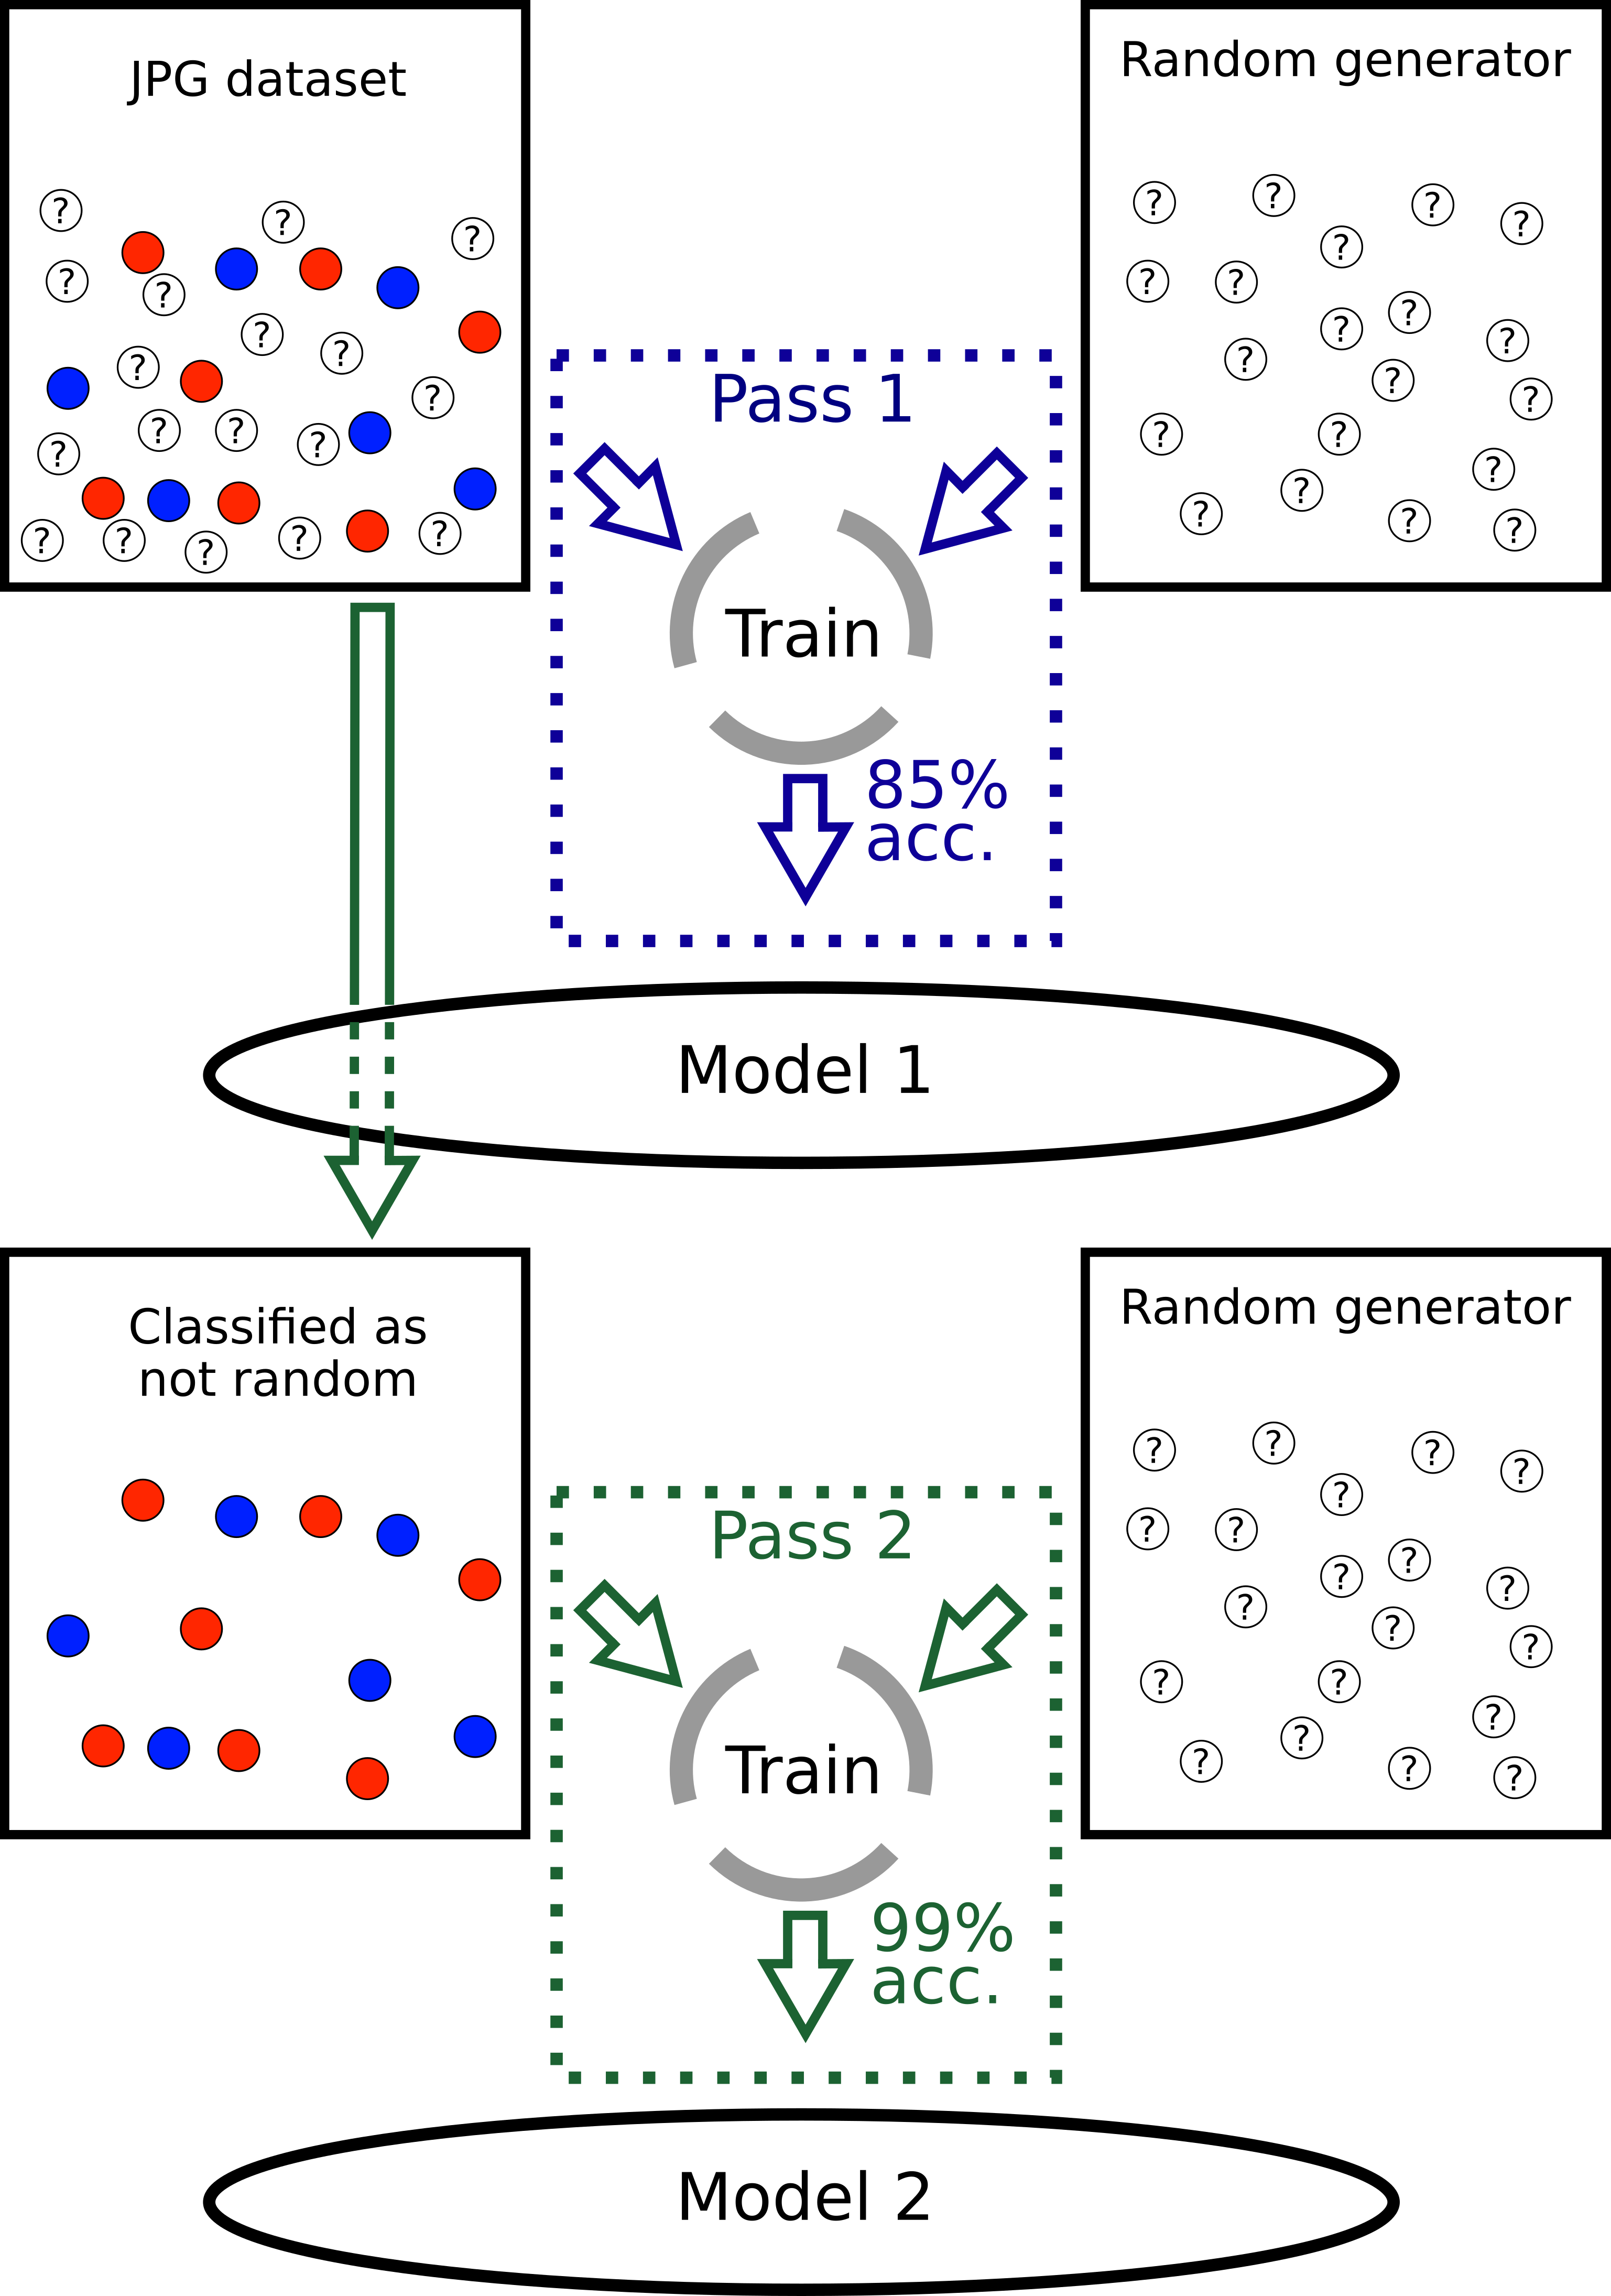
\includegraphics[width=0.5\textwidth]{content/random_measure.png}
\caption{\label{fig:randommeasure}Example of the random measure for the JPG file type. In pass 1, a model is trained to classify the data as ``random'' or ``structured'', achieving 87\% accuracy. In pass 2, another model is trained to do the same task, but the JPG blocks used are those classified as ``structured'' by model 1. As model 2 achieves an accuracy of 99\%, it validates that almost all the blocks classified as ``structured'' by model 1 are indeed not random. Then model 1 can be used to make an upper boundary estimate of the randomness of the dataset.}%
\end{figure*}

When the model training finishes, if the validation accuracy is above 98\% for a given file type, no further passes are required by that file type, as the model already can distinguish between ``random'' and ``structured'' classes for that particular file type. This will only happen on file types that have almost no random-like structures.

In the second pass, the file type dataset is filtered and only those fragments classified as ``structured'' in the first pass are used in the second pass. The random generator does not require similar filtering. If in the second pass the accuracy is above 98\%, it means that the first pass successfully selected samples that have almost no random-like structures. In that case, the model of the first pass can then used in the original dataset, giving a count of how many fragments are correctly identified as ``structured''.

The complexity of using two passes to measure the false positive rate of the model of the first pass is necessary because a direct comparison using the sample labels is insufficient for validation. From the labels, it is possible to know if the sample came from the Govdocs1 dataset or from the random generator. But, to perform validation, it would be necessary to have previous knowledge of which of the samples from the Govdocs1 dataset should be classified as ``random'' and which should be classified as ``structured''. This piece of information is unknown until the model of the first pass is trained.
